\documentclass{subfiles}

\begin{document}

\begin{figure*}
    \centering
    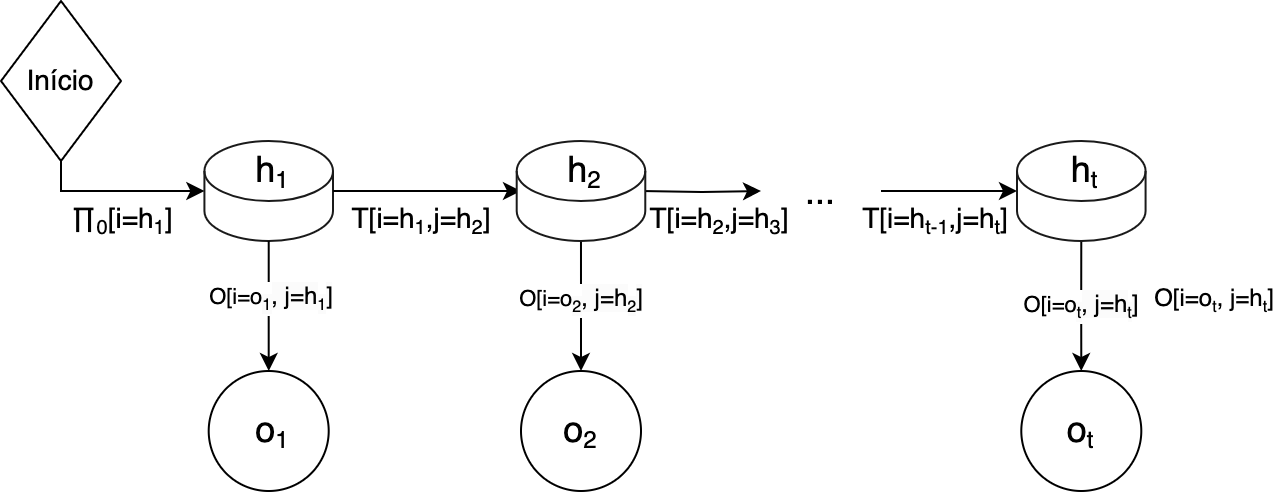
\includegraphics[width=\linewidth]{seq_hmm.png}
    \caption{Na visualização sequencial de um \textit{Modelo Oculto de Markov}, o primeiro estado oculto é sorteado com a probabilidade presente na i-ésima coluna do vetor $\Pi_0$. Em seguida é sorteado o primeiro símbolo observável com probabilidade da coluna $j$ que corresponde o estado sorteado $h_1$ e linha $i$ correspondente ao símbolo observável $o_1$ na matriz $O$. O próximo estado é selecionado com probabilidade com a linha $i$ correspondente à $h_1$ e coluna $j=h_2$. O padrão se repete até um período $t$}
    \label{fig:seq_hmm}
\end{figure*}

Imagine uma sequência $(e_i)_{i=1}^t$ gerada por processo estocástico à moda da \textit{Cadeia de Markov} como já vimos na seção anterior, adicionando um elemento: os estados não explícitos nas sequências, cada estado emite uma símbolo observável $o_i$, com o detalhe que a cada estado tem a sua própria distribuição de probabilidade para esses símbolos, como ilustrada na figura. Chama-se de \textit{Modelo Oculto de Markov} o processo estocástico que gera tais sequências de elementos observáveis.

Perceba que a \textit{Cadeia de Markov} pode ser interpretada como um \textit{Modelo Oculto de Markov} degenerado, no qual o espaço dos símbolos observáveis é o próprio espaço dos estados e cada estado emite com probabilidade $1$ elemento que o representa.

\subsection{Modelo das Urnas e Bolas}

\begin{figure}
    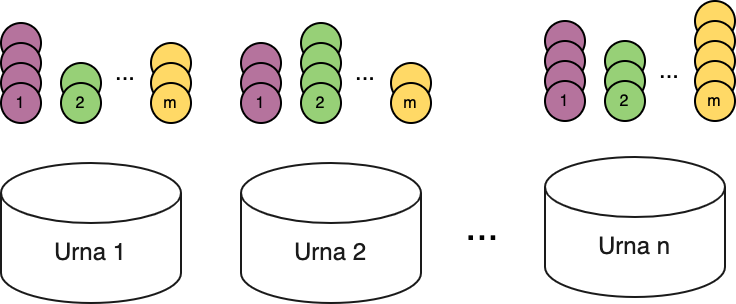
\includegraphics[width=\linewidth]{urns_balls.png}
    \caption{Os elementos do sorteio são $n$ urnas com bolas de $m$ cores diferentes organizadas de forma que cada urna tem a sua proporção de bolas em cada cor}
    \label{fig:urn_ball}
\end{figure}

Vamos ilustrar o \textit{Modelo Oculto de Markov} com um exemplo que leva elementos apresentado por Jack Ferguson. Imagine um sorteio seriado organizado com $n$ urnas cada uma com sua própria distribuição de bolas com $m$ cores diferentes e um sorteador, como ilustrado na figura \ref{fig:urn_ball}.

Este sorteador irá escolher secretamente uma urna e a partir desta urna irá sortear com reposição uma bola e somente esta bola será revelada. No próximo sorteio a escolha da próxima urna dependerá da primeira, como é feito nas \textit{Cadeias de Markov}, e desta urna será apresentada a segunda bola. Assim se repete o processo.

Note que se o caso fosse de apenas dois estados fossem observados como uma cara ou coroa, da mesma forma que Rabiner (1989) \autocite{Rabiner:1989tut} ilustra, um modelo contendo apenas um estado que entregasse a mesma distribuição das observações entre cara e coroa, seria mais informativo que um modelo com complexas relações entre urnas e bolas.

\subsection{Parâmetros do Modelo}

Além de todos os elementos já presentes na \textit{Cadeia de Markov}:
\begin{itemize}
    \item quantidade de estados $h_i$ da cadeia $n \in \mathbb{N}$;
    \item distribuição de probabilidade inicial $\Pi_0 \in \mathbb{R}^n$; 
    \item matriz probabilidade de transferência $T \in \mathbb{R}^{n \times n}$
\end{itemize}
são adicionados os elementos referentes aos símbolos visíveis
\begin{itemize}
    \item quantidade de símbolos observáveis $o_i$ emitido pelo processo $m \in \mathbb{N}$
    \item matriz distribuição de probabilidade dos símbolos observáveis em cada estado $O \in \mathbb{R}^{m \times n}$
\end{itemize}
A iteração desses elementos estão representados na figura \ref{fig:seq_hmm} que ilustra a operação sequencial de um processo modelado por um \textit{Modelo Oculto de Markov}

Apesar de um dado processo que se comporte como um \textit{Modelo Oculto de Markov} esteja bem descrito com esses elementos, mais a frente será apresentada uma representação alternativa que será capaz de responder as principais perguntas a serem feitas sobre um dado processo que só se sabe das sequências de símbolos observáveis.

\subsection{Principais perguntas ao Modelo}

Dentre as possíveis perguntas que podem ser feitas a cerca do funcionamento do modelo, serão destacadas 3 perguntas essenciais que Rabiner (1989) \autocite{Rabiner:1989tut}

\begin{enumerate}
    \item Dada uma sequência de observações $(x_i)_{i=1}^t$ e um modelo $(\Pi_0, T, O)$ qual é a probabilidade do modelo emitir a sequência
    \item Dada uma sequência de observações $(x_i)_{i=1}^t$ e um modelo $(\Pi_0, T, O)$ qual é a sequência de estados ocultos $(y_i)_{i=1}^t$ que melhor descreve as observações feitas
    \item Como ajustar os parâmetros do modelo $(\Pi_0, T, O)$ para maximizar a probabilidade de emitir as sequências de símbolos observados.
\end{enumerate}
A primeira pergunta já teve uma investigação inicial para o caso da \textit{Cadeia de Markov}. É importante avaliar essas probabilidades para se fazer comparações entre modelos. Em contraste ao caso da cadeia, a primeira pergunta não é trivialmente calculado de forma eficiente para os modelos ocultos. O complicador é que se o modelo tiver $m$ possíveis estados e $t$ termos, haverá $m^t$ possíveis sequências de estados ocultos a serem avaliados para se calcular tal probabilidade. Um algoritmo muito mais eficiente para essa estimativa é através do Procedimento \textit{Backward-Forward} de Baum (1967) \autocite{Baum:1967AnIW}. Rabiner estima que a complexidade desse procedimento é de $O(n^2t)$. Também será exposto na seção seguinte uma solução baseada na características espectrais do modelo como apresentado por Hsu, et al. (2012) \autocite{Hsu:20121460}

Já a segunda pergunta, pode ser resolvida pelo \textit{Algoritmo de Viterbi} \autocite{Viterbi:1967EBFC} que escolhe o estado seguinte que maximiza o $P((h_i)_{i=1}^t \vert (o_i)_{i=1}^t, ((\Pi_0, T, O)))$. A complexidade computacional do algoritmo também é $O(n^2t)$, como estima C. Zhu\autocite{ZHU:202127}. Essa análise permite avaliar as estruturas do modelo. Quando o modelo está sendo treinado, os parâmetros a serem aprendidos são criados sem significado explícito, esta avaliação nos permite entender que estados ocultos capturam que aspectos do modelo. É importante destacar que, apesar da popularidade de \textit{Viterbi} não existe uma métrica única para avaliar essa resposta, o próprio Rabiner \autocite{Rabiner:1989tut} ilustra outro critério, escolher a sequência de estados ocultos os quais cada estado é individualmente o mais provável dado o tempo, porém o autor também aponta que é possível que tal abordagem possa chegar em sequências possuem estados ocultos consecutivos com probabilidade de transferência nula entre eles.

A terceira finalmente a terceira pergunta interessa especialmente para Rabiner, pois a ele interessa alguma solução para melhorar a qualidade das previsões do modelo iterativamente que interessa para métodos como o de \textit{Baum-Weich}, não interessa para o algoritmo espectral de Hsu.

% Apesar do foco deste trabalho sejam os \textit{Modelos Ocultos de Markov}, a seção anterior nos deu algumas ferramentas importantes para compreender o tema principal. É chamado de \textit{Modelo Oculto de Markov} o processo estocástico no qual são observados elementos que são sorteados de acordo com o estado de uma \textit{Cadeia de Markov}.



\end{document}
